\documentclass[a4paper,12pt]{article}
\usepackage[margin=0.7in]{geometry}
\usepackage[latin1]{inputenc}
\usepackage[english]{babel}
\usepackage{amsmath}
\usepackage{cases}
\usepackage[makeroom]{cancel}
\usepackage{amsmath,tabu}
\usepackage[fleqn]{mathtools}
\usepackage[fleqn]{amsmath}
\usepackage{bm}
\usepackage{tikz}
\usepackage{enumitem}
\usepackage{wrapfig}
\usepackage{graphicx}
\usepackage{siunitx}
\usepackage{microtype}
\usepackage{array,tabularx}
\usepackage{float}

\title{\textbf{PRECEPT 3}: Heat rejection system}
\author{Rossi Andrea 875272}
\date{}

\newcommand{\celsius}[0]{\,^{\circ}C}
%\newcommand{\bar}[0]{\,bar}
\newcommand{\kjkg}[0]{\,\frac{kJ}{kg}}
\newcommand{\kjkgk}[0]{\,\frac{kJ}{kg \cdot K}}
\newcommand{\kgmcube}[0]{\,\frac{kg}{m^3}}
\newcommand{\mcubekg}[0]{\,\frac{m^3}{kg}}
\newcommand{\kgs}[0]{\,\frac{kg}{s}}
\newcommand{\kw}[0]{\,kW}
\newcommand{\mw}[0]{\,MW}
\newcommand{\msquare}[0]{\,m^2}
\newcommand{\m}[0]{\,m}
\newcommand{\wmsquareK}[0]{\,\frac{W}{m^2 \cdot  K}}
\newcommand{\gonkg}[0]{\,\frac{g_\hoo}{kg^{dry}_{air}}}
\newcommand{\md}[0]{Mollier diagram }
\newcommand{\hoo}[0]{{H_2O}}
\newcommand{\apc}{ASHRAE Psychrometric Chart }

\ExplSyntaxOn
  \cs_new_eq:NN \calc \fp_eval:n
\ExplSyntaxOff
\newcommand*{\formatNumber}[2][]{\num[%
  round-mode=places,% Round output to specified number of places
  round-precision=2,% Round-precision is 3
  output-decimal-marker={.},% Use , as decimal marker
  #1% Other options
  ]{\calc{#2}}}

\newcommand{\pointdatatable}[5]{
\begin{center}
\tabulinesep=1.2mm
\begin{tabu}{|c|c|c|c|}
\hline
$ T_{#1} $ & $ p_{#1} $ & $ h_{#1} $ & $ s_{#1} $\\ \hline
$ \formatNumber{#2} \celsius $ & $ \formatNumber{#3} \,bar $ & $ \formatNumber{#4} \kjkg $ & $ \formatNumber[round-precision=4]{#5} \kjkgk $\\ \hline
\end{tabu}
\end{center}
}

\renewcommand{\thesubsection}{\thesection.\Alph{subsection}}


%\newenvironment{conditions*}
%  {\par\vspace{\abovedisplayskip}\noindent
%   \tabularx{\columnwidth}{>{$}l<{$} @{${}={}$} >{\raggedright \arraybackslash}X}}
%  {\endtabularx\par\vspace{\belowdisplayskip}}
\newenvironment{conditions}[1][where:]
  {#1 \begin{tabular}[t]{>{$}l<{$} @{${}={}$} l}}
  {\end{tabular}\\[\belowdisplayskip]}

%
%
%
%
%
%
%
%
%
%
%
\begin{document}
\maketitle

The aim of this precept is to design a water-cooled condenser that transfers heat from a steam cycle to the environment. In a generic power plant, $270 \kgs$ of superheated steam of temperature $T=565 \celsius$ and pressure $p=100\, bar$ are first expanded in a turbine with an isoentropic efficiency of $88\%$ and are subsequently introduced in a shell and tube water condenser at $0.05\, bar$. In particular is required:

\begin{itemize}
\item QUESTION 1: Design of an open-circuit shell and tube water condenser
It is requidered to:
\begin{enumerate}[label=\Alph*.]
\item Calculate the cooling water mass flow rate;
\item Calculate the total heat transfer surface area;
\item Calculate the number and the length of the tubes;
\item Calculate, approximately, the dimensions of the water condenser, knowing that the inlet mean velocity of the steam is 200 m/s; 
\item Calculate the pressure drop at cooling water side. 
\end{enumerate}
%%%%%%%%%%%%%%%%%%%%%%%%%%%%%%%%%%%%%%%%%%%%%%%%%%%%%%%%%%%%%%%%%%%%%
\item QUESTION 2: Design of an open-circuit evaporative cooling tower 
It is requidered to:
\begin{enumerate}[label=\Alph*.]
\item Calculate the new condensation pressure and the mechanical power loss of the steam turbine; 
\item Calculate the pressure drop;
\item Calculate the steam mass flow rate discharged to the environment;
\item Calculate the air mass flow rate and L/G (Liquid/Gas) ratio;
\item Calculate the cooling tower surface area;
\item Calculate the total consumption of the water, knowing that:
\begin{itemize}
\item The fraction of the lost water due to the drag in the cooling tower is $0.2\%$ of the re-circulating water to the condenser;
\item The maximum concentration of salts in the water is smaller than three times of the initial value (related to the makeup water) 
\end{itemize}
\end{enumerate}
\end{itemize}

\newpage


\section{Solution: QUESTION 1}

\subsection{Calculation of the cooling water mass flow rate}
To evaluate the mass flow rate of water an energy balance is needed. Before to proceed to write down the balance is necessary to now the thermodynamic condition at each point involved, in particular at the inlet and the outlet of the steam turbine and at the inlet and the outlet of the heat exchanger.
\begin{figure}[h]
	\centering
    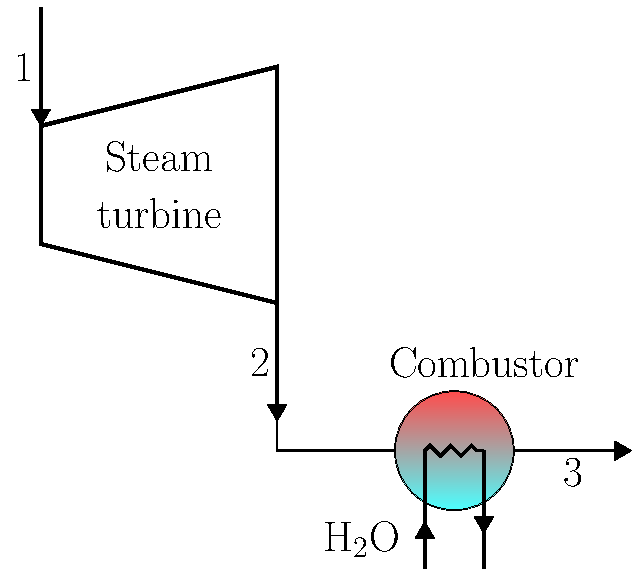
\includegraphics[scale=0.7]{st_fig.pdf}
    \caption{Turbine and combustor scheme.}
\end{figure}
We know temperature and pressure at point 1 and only pressure at point 2. From both $p$ and $T$ of the same point with \md we can evaluate all the other thermodynamic properties, in particular the elthalpy $h$.
Immediately we can find enthaply and entropy of point 1:
\begin{align*}
h_1 &= h(p_1, T_1) = 3539.3 \kjkg\\
s_1 &= s(p_1, T_1) = 6.8034 \kjkgk
\end{align*}
So point 1 properties are:
\pointdatatable{1}{565}{100}{3539.33595252716}{6.80339260873308}
From definition of isoentropic efficiency of the turbine we know that:
\begin{equation}
\label{eq:eta_turbine_iso}
\eta_T^{isoentropic} = \frac{h_1-h_2}{h_1-h_2^{IS}} = 88\%
\end{equation}
We can get $h_2^{IS}$ considering an \emph{isoentropic process} between 1 and $2_IS$ so:
\[\begin{cases}{}
p_2^{IS} = p_2 = 42 \,bar \\ 
s_2^{IS} = s_1 = 6.61 \kjkgk
\end{cases}\]
Now we can obtain from \md $h_2^{IS} = h(p_2^{IS},\ s_2^{IS}) = 2074.0 \kjkg$.
\\Reversing equation \ref{eq:eta_turbine_iso} we can get $h_2$:
\begin{equation}
h_2=h_1-\eta_T^{iso} \cdot \left(h_1 - h_2^{IS} \right) = 2249.9 \kjkg
\end{equation}
With \md we finally evaluate $s_2 = s(p_2,\ h_2)$ and $T_2 = T(p_2,\ h_2)$ of point 2:
\pointdatatable{2}{32.8754895237602}{0.05}{2249.86324200829}{7.37797750921982}
Of point 3 at the outlet of the condenser we know the pressure $p_3=p_2=p_{cond} = 0.05\, bar$; considering that the condenser gives out a \emph{saturated liquid} flow we can evaluate properties of point 3:
\pointdatatable{3}{32.8754895237602}{0.05}{137.765118988491}{0.476253789505102}
Now we can finally write the energy balance of the condender:
\begin{equation}
\label{eq:energy_balance_condenser}
\dot{Q}_{steam} = 
\dot{m}_{steam} \cdot (h_2-h_3) =
\dot{m}_{H_2O} \cdot \overline{c}_{p_{H_2O}} \cdot (T_{H_2O}^{OUT} - T_{H_2O}^{IN}) = \dot{Q}_{H_2O} = 
\formatNumber{570.266493215347} \kw
\end{equation}
We know $T_{H_2O}$ at the inlet and the outlet, so we can estimate a medium value of $\overline{c}_{p_{H_2O}}$ between the two temperatures:
\begin{align*}
c_p(T_{H_2O}^{OUT}) &= 
\formatNumber[round-precision=3]{4.1837904904686} \kjkgk\\
c_p(T_{H_2O}^{OUT}) &= 
\formatNumber[round-precision=3]{4.19051961001919} \kjkgk\\
\overline{c}_{p_{H_2O}} &= \frac{c_p(T_{H_2O}^{OUT})+c_p(T_{H_2O}^{IN})}{2} = 
\formatNumber[round-precision=3]{4.1871550502439} \kjkgk\\
\end{align*}
Now the only unknown of equation \ref{eq:energy_balance_condenser} is $\dot{m}_{H_2O}$ that can be found refersing the formula:
\begin{equation}
\label{eq:mass_flow_rate_water1}
\dot{m}_{H_2O} = 
\frac{\dot{m}_{steam} \cdot (h_2-h_3)}{\overline{c}_{p_{H_2O}} \cdot (T_{H_2O}^{OUT} - T_{H_2O}^{IN})} = 
\formatNumber[round-precision=1]{17024.2827878481} \kgs
\end{equation}
It is also convenient to evaluate volume flow rate:
\begin{equation}
\label{eq:volume_flow_rate}
\dot{V}_{H_2O} = \frac{\dot{m}_{H_2O}}{\overline{\rho}_{H_2O}} = 
\formatNumber{17.0489778573119} \kgmcube
\end{equation}
where $\overline{\rho}_{H_2O}$ is evaluated in mean temperature between in and out, $\overline{T} = 18 \celsius$.

\subsection{Calculation of the total heat transfer surface area;}
\label{sec:heat_transfer_area}
We know the thermal power at condenser from equation \ref{eq:energy_balance_condenser}. We can write it as heat exchanged by a certain total surface $A_{TOT}$ with convection and conduction:
\begin{equation}
\label{eq:Q_dot_condenser}
\dot{Q}_{condenser} = U \cdot A_{TOT} \cdot \Delta T_{mean log}
\end{equation}
\begin{conditions}
 U     				 &  global heat transfer coefficient;\\
 A_{TOT}   			 &  total area of heat transfer (external wall of the tubes);  \\   
 \Delta T_{ml} &  log-mean temperature difference, defined as: 
\end{conditions}

\begin{equation}
\label{eq:deltaT_meanlog}
\Delta T_{ml} = \dfrac{\Delta T_{IN} - \Delta T_{OUT}}
{\ln \left( 
\dfrac{\Delta T_{IN}}{\Delta T_{OUT}}
\right)}
\end{equation}
\begin{conditions}
 \Delta T_{IN}  & $T_{condensation} - T^{IN}_{\hoo} 
 = T_{sat}(p_{cond}) - T^{IN}_{\hoo}$;\\[0.5em]
 \Delta T_{OUT} & $T_{condensation} - T^{OUT}_{\hoo}
 = T_{sat}(p_{cond}) - T^{OUT}_{\hoo}$;
\end{conditions}
We have every temperature so we can immediately evaluate $\Delta T_{ml}$:
\begin{equation}
\Delta T_{ml} = \formatNumber{14.5097700034933} \celsius
\end{equation}

\begin{wrapfigure}{R}{4cm}
\vspace{-0.7cm}
    \caption{Wall}
    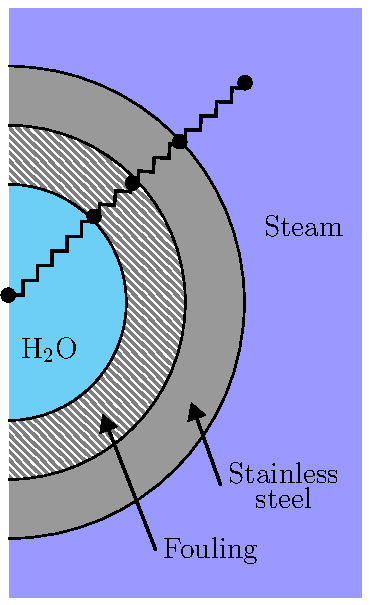
\includegraphics[scale=0.65]{resistance_fig.pdf}
\end{wrapfigure}
The only unknown is $U$. To compute it we apply the similitude with elettrical resistance; we can see each heat exchange as a resistence and all the layers together as many series resistance, and then apply series rule:
\begin{equation}
R_{TOT} = \frac{1}{U \cdot A_{TOT}}
= \sum_{i=1}^{layers} R_i
= R_{int} + R_{fouling} + R_{steel} + R_{ext}
\end{equation}

We can distinguish 4 different contributions:
\begin{itemize}
\item Convective resistance of the water $R_{int}$;
\item Conductive resistance of the fouling $R_{fouling}$;
\item Conductive resistance of the tube $R_{steel}$;
\item Convective resistance of the steam $R_{ext}$.
\end{itemize}
\begin{equation}
R_{int} = \frac{1}{h_{int} \cdot A_{int}}
 = \frac{1}{A_{ext}} \cdot \frac{1}{h_{int} \cdot \frac{A_{int}}{A_{ext}}}
 = \frac{1}{A_{ext}} \cdot \frac{1}{h_{int} \cdot 
 \frac{\cancel{\pi} D_{int} \cdot \cancel{L_{tube}}}{ \cancel{\pi} D_{ext} \cdot \cancel{L_{tube}}}}
 = \frac{1}{A_{ext}} \cdot \left( \frac{1}{h_{int}} \cdot \frac{D_{ext}}{D_{int}} \right)
\end{equation}
\begin{equation}
R_{fouling} = \frac{F.F}{A_{int}}
 = \frac{1}{A_{ext}} \cdot \frac{F.F}{\frac{A_{int}}{A_{ext}}}
 = \frac{1}{A_{ext}} \cdot F.F \cdot \frac{1}{\frac{\cancel{\pi} D_{int} \cdot \cancel{L_{tube}}}{ \cancel{\pi} D_{ext} \cdot \cancel{L_{tube}}}}
 = \frac{1}{A_{ext}} \cdot \left( F.F \cdot \frac{D_{ext}}{D_{int}} \right)
\end{equation}
\begin{equation}
R_{steel} = \frac{\ln \left( 
\dfrac{D_{ext}}{D_{int}}
\right)}{2\pi \cdot k_m \cdot L_{tube}}
 = \frac{1}{A_{ext}} \cdot \frac{\ln \left( 
\dfrac{D_{ext}}{D_{int}}
\right)}{\frac{2\pi \cdot k_m \cdot L_{tube}}{A_{ext}}}
= \frac{1}{A_{ext}} \cdot \frac{\ln \left( 
\dfrac{D_{ext}}{D_{int}}
\right)}{\frac{2\cancel{\pi} \cdot k_m \cdot \cancel{L_{tube}}}{\cancel{\pi} D_{ext} \cdot \cancel{L_{tube}}}}
= \frac{1}{A_{ext}} \cdot \ln \left(\dfrac{D_{ext}}{D_{int}} \right)\frac{D_{ext}}{2 \cdot k_m}
\end{equation}
\begin{equation}
R_{ext} = \frac{1}{h_{ext} \cdot A_{ext}}
 = \frac{1}{A_{ext}} \cdot \frac{1}{h_{ext} \cdot \frac{A_{ext}}{A_{ext}}}
 = \frac{1}{A_{ext}} \cdot \frac{1}{h_{ext} \cdot 
 \frac{\cancel{\pi} \cancel{D_{ext}} \cdot \cancel{L_{tube}}}{ \cancel{\pi}  \cancel{D_{ext}} \cdot \cancel{L_{tube}}}}
 = \frac{1}{A_{ext}} \cdot \left( \frac{1}{h_{ext}} \right)
\end{equation}
Summarizing we have:
\begin{equation}
R_{TOT} = \frac{1}{A_{ext}} \cdot \left(
\frac{1}{h_{int}} \cdot \frac{D_{ext}}{D_{int}}
+ F.F \cdot \frac{D_{ext}}{D_{int}}
+ \ln \left(\dfrac{D_{ext}}{D_{int}} \right)\frac{D_{ext}}{2 \cdot k_m}
+ \frac{1}{h_{ext}}
\right)
= \frac{1}{A_{ext}} \cdot r_{EQ} = \frac{1}{U \cdot A_{ext}}
\end{equation}
The only missing data of $r_{EQ}$ if the convective heat transfer coefficient of water($h_{int}$). We can estimate through the the Nusselt number, dimensionless number that represents the weight of convection compared to only conduction
\begin{equation}
\label{eq:nusselt_def}
Nu = \frac{h_{int}}{k_{\hoo}} \cdot D_{int}
\end{equation}
Under the assumptions of the flow in smooth pipes, turbulent flow (check with the Reynolds number) and heating flow, the Nusselt number can be estimated through the correlation of Dittus Boelter:
\begin{equation}
Nu = 0.023 \cdot Re^{0.8} \cdot Pr^{0.4}
\end{equation}
\begin{equation}
\begin{conditions}
\label{eq:reynolds}
 Re & $\frac{\rho_{\hoo} \cdot w_{\hoo} \cdot D_{int}}{\mu_{\hoo}}
 = \formatNumber{43194.7856273791}$;\\[0.5em]
 Pr & $\frac{\mu_{\hoo} \cdot c_{p_{\hoo}}}{k_{\hoo}}
 = \formatNumber[round-precision=3]{7.96955177896421}$;
\end{conditions}
\end{equation}
To evaluate this previous dimensionless number we have used medium values of the main properties required like $\rho$, $\mu$, $c_p$ and $k$.
Now the Nusselt number is $Nu = \formatNumber{17.0077339278223}$. Reversing equation \ref{eq:nusselt_def} we finally get convective heat transfer coefficient of the water:
\begin{equation}
h_{int} = Nu \cdot \frac{k_{\hoo}}{D_{int}} = \formatNumber{8512.2447541249} \wmsquareK
\end{equation}
The only missing value to calculate the global heat transfer coefficient U was $h_{int}$ so:
\begin{equation}
\frac{1}{A_{ext}} \cdot r_{EQ} = \frac{1}{U \cdot A_{ext}}
\quad \Rightarrow \quad
U = \frac{1}{r_{EQ}} = 
\formatNumber{2123.08634088264} \wmsquareK
\end{equation}
At the end from \ref{eq:Q_dot_condenser} we finally obtain the total surface $A_{TOT}$ of the condenser:
\begin{equation}
A_{TOT} = \frac{\dot{Q}_{condenser}}{U \cdot \Delta T_{mean log}}
= \formatNumber{18511.843500699} \msquare
\end{equation}







\subsection{Calculation of the number and the length of the tubes;}
Assuming that the layout of the condenser is as in the figure 2, the tubes are all the same and the velocity of the water is constant inside them, the volumetric flow rate can be expressed as a function of number of tubes: 
\begin{equation}
\dot{V}_{\hoo} = w_{\hoo} \cdot A_{tube} \cdot N_{tubes} = w_{\hoo} \cdot  N_{tubes} \cdot \pi \frac{(D_{ext}-2t)^2}{4}
\end{equation}
But $\dot{V}_{\hoo}$ is calculated before in equation \ref{eq:volume_flow_rate}, so we can reverse the equation and find the number of tubes because the other parameters are known.
\begin{equation}
N_{tubes} = \frac{\dot{V}_{\hoo}}{w_{\hoo} \cdot A_{tube}} \approx
\formatNumber[round-precision=0]{23127.4587739651} 
\end{equation}

From the total surface of the condenser and the number of tubes we can calculate the serface of the single tube. Moreover the single tube is schematized as a cilinder, so we can compare the two different calculation tu evaluate the lenght of a sigle tube:
\begin{numcases}{}
S_{tube} = \frac{A_{TOT}}{N_{tubes}}\\
S_{tube} = \pi \cdot D_{ext} \cdot L_{tube}
\end{numcases}
\begin{equation}
\quad 
\Rightarrow
\quad
L_{tube} = \frac{A_{TOT}}{N_{tubes}} \cdot \frac{1}{\pi \cdot D_{ext}}
= \formatNumber{12.1325638957687} \m
\end{equation}

\subsection{Calculation of, approximately, the dimensions of the water condenser; }
The sizing of the water cooled condenser must take into account the dimensions, such as the length, the width and the height, but also the length and the arrangement  of tubes inside it. 
To have an approximation of the size we assume that the condenser is inside a parallelepid of size $w \times l\times h$. 
From the total volumetric flow rate of the steam and its velocity we can estimate the front surface of the condenser:
\begin{equation}
A_{front} = w \times l = \frac{\dot{V_{steam}}}{w_{steam} \cdot \rho_{steam}}  = \formatNumber{33.1691906743412} \msquare
\end{equation}
We have used properties ($\rho$) at the outlet of the steam turbine, the point 2.
For a good design point of view is important to have a  ratio between w and l close to one to have approximately a square face. To ensure to reach the proper ratio we can bend multiple times the tube.
With no bending:
\begin{equation}
l = L_{tube} 
\quad \Rightarrow\quad
w = \frac{A_{front}}{l} 
= \formatNumber{2.73389787676363} \m
\end{equation}
In this case the ratio is equal to: $
l/w = \formatNumber{4.43782629881228}$
It is no proper to use no bended tubes so we try with 1 bend or more untill we reach a good ratio. With 1 bend we have:
\begin{equation}
l = \frac{L_{tube}}{2}
\quad \Rightarrow\quad
w = \frac{A_{front}}{l} 
= \formatNumber{5.46779575352727} \m
\end{equation}
In this case the ratio is equal to: $
l/w = \formatNumber{1.10945657470307}$

Now we must compute the third dimention. We must consider tubes arrangement that are represented in figure \ref{fig:tubes_arrangement} in a equilateral triangular lattice.
\begin{figure}[h]
\label{fig:tubes_arrangement}
	\centering
    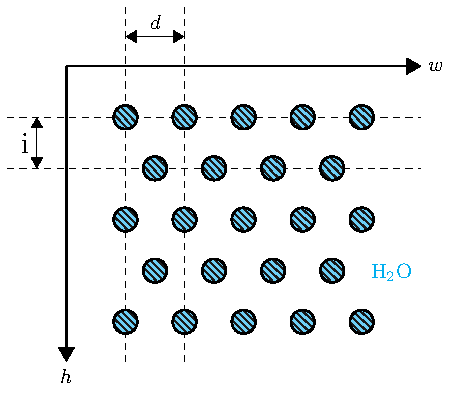
\includegraphics[scale=1]{tubes_fig.pdf}
    \caption{Tubes arrangement}
\end{figure}
Considering one time bended tubes we see a number of section doubled respect to the total number of tubes, in particular: $N_{section}=2 \cdot N_{tubes}=\formatNumber[round-precision=0]{46254.9175479301}$.
The section are separated one to each other by a distance of $d=1.8 \cdot D_{ext}$ so the number of section per each row is $N^{section}_{per\ row} = w/d = $. Directly come from this that the number of rows is:
\begin{equation}
N_{row} = \frac{N_{section}}{N^{section}_{per\ row}} = 
\frac{N_{section}}{w/d} = 
\formatNumber[round-precision=0]{319.769786971989} \, \text{rows}
\end{equation}
Considering that that distance between each row is the height of the single equilateral triangle equal to $i=\sqrt{3}/2 \cdot d$, the total height of the condenser is simply:
\begin{equation}
h = N_{row} \cdot i =  N_{row} \cdot \frac{\sqrt{3}}{2} \cdot d = 
\formatNumber{10.4679070856822} \m
\end{equation}




\subsection{Calculation of the pressure drop at cooling water side.}
\label{sec:pressur_drop_A}
The pressure drop at cooling water side, considering the steady state conditions and incompressible fluid, is evaluated as:
\begin{equation}
\Delta p = f \cdot \frac{L_{tube}}{D_{IN}} \cdot \frac{w_{\hoo}^2}{2g} =
\formatNumber{4.78826565838844} \m \text{\ of\ }  \hoo
\end{equation}
where f is the friction factor, calculated as a function of the Reynolds number estimated in equation \ref{eq:reynolds} and is equal to 
$f = 0.184 \cdot Re^{-0.2} = \formatNumber[round-precision=4]{0.0217636412497489}$
%
%
%
\newpage
\section{Solution: QUESTION 2}
The heat of the condensation, $\dot{Q}_{COND}$ previously calculated, is now transferred to the environment trough an \emph{evaporative cooling tower}. This kind of design is preferred respect to transfer heat directly to air in case it is not available a large quantity of water. Indeed using a semi-closed cycle for the water flux requires a relatively small amount of mass flow rate of fresh water respect to shell and tube condenser and is it a relatively simpler, cheaper and more efficient solution respect to air cooled condenser. 
Due to the heat a small quantity of water evaporates, few really small droplets are carried out with wet air, and due to impurity, in water is present some fraction of solids piled up at the bottom of the tower. All this quantity must be replaced with fresh new water. 

\subsection{Calculation of the new condensation pressure and the mechanical power loss of the steam turbine;}

If in question 1 we know saturation pressure that let us to use the \emph{mean log method} to evaluate power exchanged in the condensator, now the temperature at which water comes out from the condenser is unknown making mean log method inneffective. So in this case we must procede in an iterative process and apply \emph{NTU method}. 
The complete cycle is represented in figure \ref{iterative_scheme}.
Moreover we now assume that the mass flow rate of water $\dot{m}_{\hoo}$ is equal to $0.9$ of the previous value, in particular:
\begin{equation}
\dot{m}_{\hoo}^{NEW} = 0.9 \cdot \dot{m}_{\hoo} = \formatNumber{15321.8545090633} \kgs
\end{equation}
Starting with a likely guess value for $p_{cond}$ we procede in the same way as question 1, evaluating the thermodynamic properties of point 2 at the outlet of the turbine and of point 3 at the outlet of the condenser. Then we estimate $\dot{Q}_{cond}$ from $h_2$ and $h_3$, and the variation of temperature that the water flow must get to exchange that heat and conseguentially the temperature of $\hoo$ at the outlet of condender. In fact from data we can get the inlet temperature from \apc knowing that the dry bulb temperature of $T_{DB}=16 \celsius$ and the relative humidity $\phi=50\%$ are assigned. 
\begin{equation}
T_\hoo^{IN} = T_{WB}(T_{DB},\phi) + 7 \celsius = \formatNumber{10.45090571708937} \celsius + 7 \celsius = \formatNumber{10.45090571708937+7} \celsius
\end{equation}
Proceding in the same way as question \ref{sec:heat_transfer_area} we compute the global heat transfer coefficient $U$.
Now we can apply \emph{NTU method}; NTU is defined as
\begin{equation}
NTU = \text{number of thermal unit} = \frac{U \cdot A_{TOT}}{\dot{m}_\hoo \cdot c_{p_\hoo}}
\end{equation}
Insteam the effectiveness $\varepsilon$ equals to:
\begin{equation}
\label{eq:NTU_epsilon}
\varepsilon \stackrel{\text{def}}{=} \frac{\dot{q}}{\dot{q}_{MAX}} = 
\dfrac{\cancel{\dot{m}_\hoo} \cdot \cancel{c_{p_\hoo}} (T_{OUT}-T_{IN})}
	  {\cancel{\dot{m}_\hoo} \cdot \cancel{c_{p_\hoo}} (T_{COND}-T_{IN})} = 1-e^{-NTU}
\end{equation}
Reverting equation \ref{eq:NTU_epsilon} we get a relationship between NTU that we have already compute and $T_{COND}$ that we have indirectly guessed at the beginning we we have supposed a value for $p_{COND}$.
Now we have obtained a new value of $p_{COND}$ that we can compare with the starting value. If their different is small enough we can stop and we have finally a realistic value of $p_{COND}$ otherwise we proceed again in the loop using this new value untill we reach our stopping condition. If the starting guess is not so far from the solution, our strategy converg quite quickly to the solution. We find that  $p_{COND} = \formatNumber{0.062939626246445} \,bar$.
\newpage
\begin{figure}[H]
    \caption{Iterative process to compute $p_{cond}$}
	\centering
    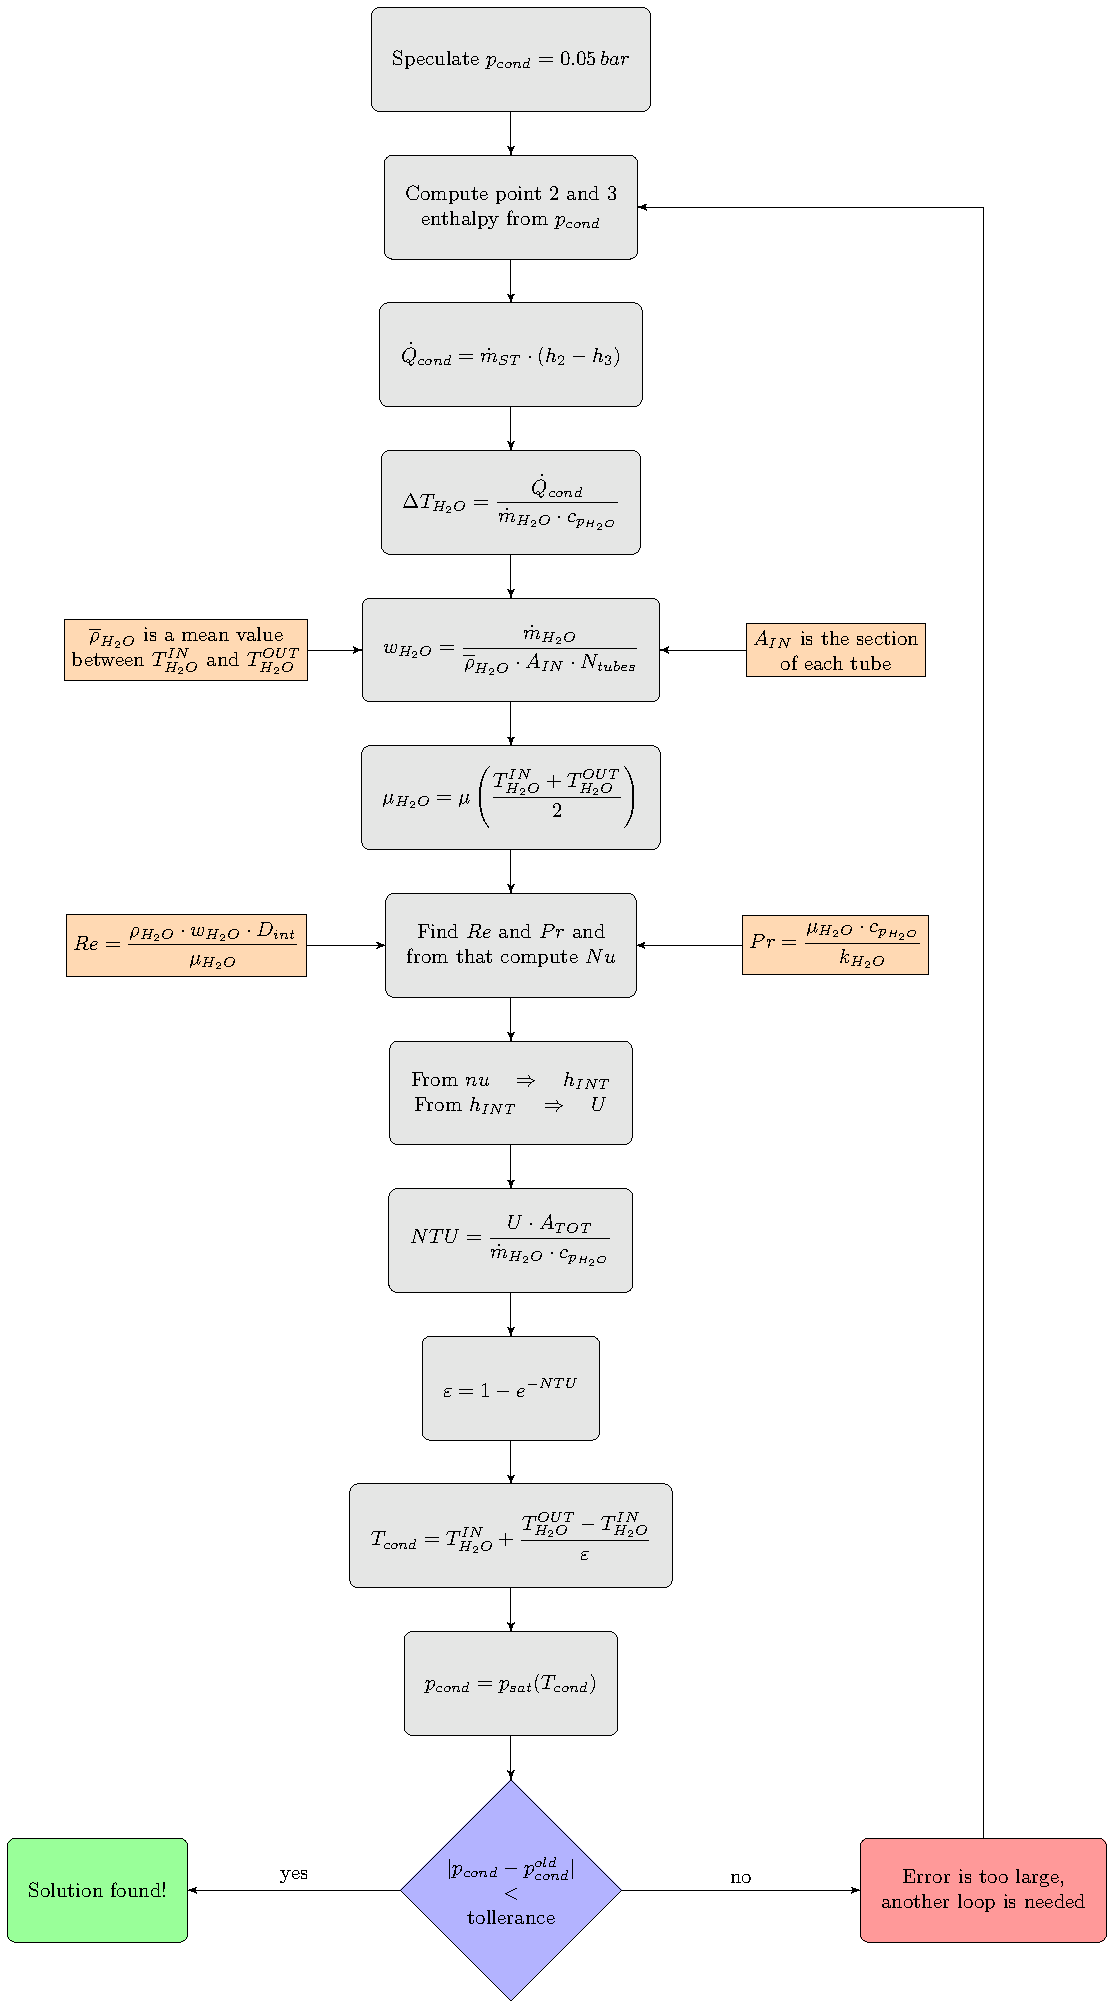
\includegraphics[width=\textwidth,height=\textheight,keepaspectratio]{diagram_fig.pdf}
	\label{iterative_scheme}
\end{figure}

With new value of condensation pressure, the thermodynamic conditions of the steam at outlet of the turbine are also changed and are evaluated in the last cycle; as a consequence, the mechanical power of the steam turbine changes and we can evaluate the pressure drop of the case B as:
\begin{equation}
\Delta P = \dfrac{ \cancel{\dot{m}_{ST}} \cdot (\cancel{h_1} - h_2^{A})  
					 -  \cancel{\dot{m}_{ST}} \cdot (\cancel{h_1} - h_2^{B})  }
				 { \cancel{\dot{m}_{ST}} \cdot (h_1 - h_2^{A})}  = 
\dfrac{ h_2^{B} -  h_2^{A}  }
	  { h_1 - h_2^{A}} 
= \formatNumber{1.78829240712947} \%
\end{equation}
%
%
%
%
\subsection{Calculation of the pressure drop;}
The pressure drop at cooling water side, considering the steady state conditions and incompressible fluid, is evaluated like question \ref{sec:pressur_drop_A} as:
\begin{equation}
\Delta p = f \cdot \frac{L_{tube}}{D_{IN}} \cdot \frac{w_{\hoo}^2}{2g} =
\formatNumber{3.86449162135387} \m \text{\ of\ }  \hoo
\end{equation}
where f is the friction factor, calculated as a function of the Reynolds number and is equal to 
$f = 0.184 \cdot Re^{-0.2} = \formatNumber[round-precision=4]{0.0216502094202132}$
%
%
%
%
\subsection{Calculation of the steam mass flow rate discharged to the environment;}
In order to calculate the air mass flow rate, it is necessary to evaluate the properties of the air between inlet and outlet of the cooling tower, as shown in the following table: 
\begin{center}
\tabulinesep=1.2mm
\begin{tabu}{|l|c|c|c|c|c|c|}
\hline
   & $ T_{D.B.} $ & $ p_{W.B.} $ & $ \varphi $ & $ \chi $ & $ h^{dry}_{air}$ & $ v^{dry}_{air}$\\ \hline
IN & $ \formatNumber{16} \celsius $ & $ \formatNumber{10.4509057170894} \celsius $ & $ \formatNumber{50} \% $ & $ \formatNumber{0.005631979*1000} \gonkg $ & $ \formatNumber{30.348} \kjkg $ & $ \formatNumber{0.82569566757} \mcubekg $\\ \hline
OUT & $ \formatNumber{24} \celsius $ & $ \formatNumber{24} \celsius $ & $ \formatNumber{100} \% $ & $ \formatNumber{0.018881104*1000} \gonkg $ & $ \formatNumber{72.168} \kjkg $ & $ \formatNumber{0.853434} \mcubekg $\\ \hline
\end{tabu}
\end{center}
\begin{conditions}
D.B.     		&  dry bulb (temperature or pressure);\\
\varphi			&  relative humidity;  \\   
\chi 			&  specific humidity; \\
h^{dry}_{air}   &  enthalpy of dry air; \\
v^{dry}_{air}   &  specific volume of dry air;
\end{conditions}
With energy balance equation over the condenser power to dissipate and air that increase relative humidity we get:
\begin{equation}
\dot{Q}_{cond} = \dot{m}^{dry}_{air} \cdot (h_{OUT} - h_{IN})
\quad \Rightarrow \quad
\dot{m}^{dry}_{air} = \dfrac{\dot{Q}_{cond}}{h_{OUT} - h_{IN}}
= \formatNumber{13672.8433579543} \kgs
\end{equation}
%
%
%
%
\subsection{Calculation of the air mass flow rate and L/G (Liquid/Gas) ratio;}
The steam mass flow rate of water that evaporate is calculated by the difference of the specific humidity from inlet to outlet of the cooling tower: 
\begin{equation}
\dot{m}^{evap}_\hoo = \dot{m}^{dry}_{air} \cdot (\chi_{OUT} - \chi_{IN})
= \formatNumber{181.153210754956} \kgs
\end{equation}
Then the ratio Liquid/Gas is given by the ratio between the liquid (water) and gaseous (air) fraction circulating in the cooling tower: 
\begin{equation}
\dfrac{L}{G} = \dfrac{\dot{m}_\hoo }{\dot{m}^{dry}_{air}} = 
\frac{ \formatNumber{15321.8545090633} \kgs}{ \formatNumber{13672.8433579543} \kgs}
= \formatNumber{1.12060484479621}
\end{equation}
\subsection{Calculation of the cooling tower surface area;}
The upper section of the tower, knowing the velocity of the air at outlet of the tower and the volume flow rate of air is given by:
\begin{equation}
A_{tower} = \dfrac{\dot{V}^{dry}_{air}}{w^{dry}_{air}} = 
\dfrac{\dot{m}^{dry}_{air} \cdot v^{dry}_{air}}{w^{dry}_{air}} 
= \formatNumber{4321.80348087125} \msquare
\end{equation}
\begin{equation}
A_{tower} = \dfrac{\pi \cdot D_{tower}^2}{4}
\quad \Rightarrow \quad
D_{tower} = \sqrt{\dfrac{4 A_{tower}}{\pi}} 
= \formatNumber{74.1801260205141} \m
\end{equation}
\subsection{Calculation of the total consumption of the water;}
As explained before some quantity of water must be replaced, in particular, mass flow rate of make up must compensate:
\begin{itemize}
\item Evaporated water;
\item Droplet drag out with the flow of air;
\item Water with high concentration of solids;
\end{itemize}
We don't know yet water taken out from the bottom of the tower. In order to evaluate that purged water we can perform the salinity balance in the cooling tower because we know that the ratio between concentration of salt in make up water and in the tower is smaller than 3;
\begin{equation}
\dot{m}_{make\ up} \cdot C_{make\ up} = (\dot{m}_{drag} + \dot{m}_{tank}) \cdot C_{tower}
\end{equation} 
\begin{conditions}
C_i    					 &  salinity ($kg_{salt}/kg_\hoo$) ;\\
C_{tower} / C_{make\ up} &  3 as assigned;  \\   
\dot{m}_{drag}			 &  $0.2/100 \cdot \dot{m}_\hoo = 
\formatNumber{30.6437090181266} \kgs$ ;  \\   
\end{conditions}
Now we can write a linear system of 2 equations where the unknowns are  $\dot{m}_{make\ up}$ and $\dot{m}_{tank}$.
\begin{numcases}{}
\label{eq:makeup_1}
\dot{m}_{make\ up} = \dot{m}_{drag} + \dot{m}_{tank} + \dot{m}_{\hoo}^{evap}\\
\label{eq:makeup_2}
\dot{m}_{make\ up} = C_{tower} / C_{make\ up} \cdot (\dot{m}_{drag} + \dot{m}_{tank})
\end{numcases}
Substituting equation \ref{eq:makeup_2} into equation \ref{eq:makeup_1} we finally get:
\begin{numcases}{}
\dot{m}_{tank} = \dfrac{\dot{m}_{\hoo}^{evap}}{C_{tower} / C_{make\ up} - 1} - \dot{m}_{drag} = \formatNumber{59.9328963593516} \kgs\\
\dot{m}_{make\ up} = \dot{m}_{drag} + \dot{m}_{tank} + \dot{m}_{\hoo}^{evap} 
=\formatNumber{271.729816132435} \kgs
\end{numcases}
As expected using cooling tower instead of shall and tube condenser $\dot{m}_{make\ up}$ is order of magnitude lower than the water needed in the question 1 as evaluated with equation \ref{eq:mass_flow_rate_water1}.

\end{document}
